\section{Evaluation}
\label{sec:eval}

In this section, we evaluate the trade-off between the performance of an implementation of a summarisation relation, the volume, and the precision of the graph summary.
In this evaluation, we consider the following statements:
\begin{itemize}
	\item $G=\left\langle V, A, l_V \right\rangle$ is a graph;
	\item the bisimulation summary of $G$ is $\mathcal{S}_{fbt} = \left\langle \mathcal{W}_{fbt}, \mathcal{B}_{fbt}, l_{\mathcal{W}_{fbt}} \right\rangle$ according to the summarisation relation $R_{fbt}$;
	\item $\mathcal{S} = \left\langle \mathcal{W}, \mathcal{B}, l_{\mathcal{W}} \right\rangle$ is a summary of $G$ according to the summarisation relation $R$; and
	\item there exists a relation $S \subseteq \mathcal{W}_{fbt} \times \mathcal{W}$ such that $R_{fbt} \sqsubseteq R$.
\end{itemize}

\subsection{Design}
\label{sec:eval:design}

We describe in this section the design of the evaluation. We first present the environment of our experimental framework. Then, we describe the dimensions of our evaluation.

\subsubsection{Environment}

The bisimulation summary $\mathcal{S}_{fbt}$ is the most precise summary of the data graph, since all incoming and outgoing (and combination of) paths in the summary do exist in the data graph $G$. In this evaluation, we use the $R_{fb}$ as the \emph{gold standard} summary of a data graph, which ensures that all outgoing paths do exist. The presented summarisation relations have been implemented using the Hadoop\footnote{Hadoop: \url{http://hadoop.apache.org/}} MapReduce framework. Our Hadoop cluster is composed of 10 machines.

\subsubsection{Evaluation Dimensions}

We present in this section three dimensions we use for evaluating a summary, i.e., the \emph{volume}, the \emph{performance} of the relation, and the \emph{precision}.

\begin{quotation}
\item[\emph{Summary volume.}]

We measure the amount of data from the gold standard summary that is compressed into the evaluated summary. To this end, we compare the volume of the summary against the volume of the gold standard. We report this comparison as the ratio  $\mathcal{S}:\mathcal{S}_{fb}$ of the former to the later.

$$
\mathcal{S}:\mathcal{S}_{fb} = \frac{\vert \mathcal{W} \vert + \vert \mathcal{B} \vert}{\vert \mathcal{W}_{fb} \vert + \vert \mathcal{B}_{fb} \vert}
$$

\item[\emph{Algorithm performance.}]

%The MapReduce implementation of the graph summarisation is composed of two separate steps:
%\begin{inparaenum}[(1)]
%\item a \emph{mapping} step, where we assign a node of the data graph to its $\sim$-equivalence class; and
%\item a \emph{edges} step, where we compute the edges of $G^\sim$.
%\end{inparaenum}
We evaluate the computational performance of a summarisation relation by analysing the CPU time\footnote{The accumulated CPU time as reported with the \texttt{CPU\_MILLISECONDS} counter of Hadoop.} on the \hyperref[step-he]{Step 3} of the graph summary computation, as described in Section~\ref{chap03:algo:edge-materialisation} for the MapReduce case. We do not report on the \hyperref[step-hn]{Step 2} because the evaluated summarisation relations have the same complexity, achieving similar times on this step.

\item[\emph{Summary precision.}]

With regards to all three classification of errors, we evaluate the precision of a summary thanks to the true and false positive edges set $TP(x)$ and $FP(x)$.
We report the precision using two measures, i.e., $P1$ and $P2$.

The measure $P1$ reflects the average number of true positive edges from a randomly selected node in the inferred graph $\mathfrak{G}(R)$. From right to left, we sum the edge precisions $Prec(R, x)$ of a node $x\in \mathcal{W}_{fbt}$, which we average by the number of nodes within $C(c)$. Finally, we average over the total number of nodes within the bisimulation summary.
$$
\begin{aligned}
P1 = & \frac{1}{\vert \mathcal{W}_{fbt} \vert} \times \sum_{c \in \mathcal{W}}{\frac{1}{\vert C(c) \vert} \times \sum_{x \in C(c)}{Prec(R, x)}} \\
\text{where}\; C(c) = & \left\lbrace x \in \mathcal{W}_{fbt} \mid (x, c) \in S \right\rbrace
\end{aligned}
$$

The measure $P2$ reflects the overall chance for a randomly selected edge in the inferred graph $\mathfrak{G}(R)$ of being a true positive.
$$
P2 = \frac{\sum_{x \in \mathcal{W}_{fbt}}{TP(x)}}{\sum_{x \in \mathcal{W}_{fbt}}{TP(x) + FP(x)}}
$$
\end{quotation}

\subsection{Datasets}
\label{sec:eval:datasets}

We use in this evaluation several datasets of various complexity. We list in the Table~\ref{tab:datasets} the datasets along with some descriptive statistics. The datasets are grouped according to their complexity into four categories, i.e., \emph{Low}, \emph{Medium}, \emph{High}, and \emph{Very High}. We determined the complexity with regards to the volume of a graph and the number of unique types and attributes it possesses.

For each dataset, we present two aspects, i.e., the \emph{schema} and the \emph{structure} of the data graph. With regards to the schema complexity, we report the number of unique edge labels $\vert \mathcal{L}^A \vert$ and the number of unique types $\vert \mathcal{L}^T \vert$ of the data graph. With regards to the structure complexity, we report the size and order of $G$ and  $\mathcal{S}_{fb}$. The order values omit the number of sink nodes, i.e., nodes without outgoing edges which includes literal nodes in the RDF data model.

The $\mathcal{S}_{fb}:G$ column reports the volume ratio of $\mathcal{S}_{fb}$ to $G$ as a percentage, where the volume is the sum of the size and order of a graph. We remark that the volume of the summary $\mathcal{S}_{fb}$ is significantly smaller than the volume of the data graph. This emphasize the performance benefits of using a summary instead of the data graph itself in an application. We note that the bigger the volume ratio, the more complex the data graph is to summarise from a structural point of view. Although the datasets \texttt{bnb} and \texttt{wb} have a similar volume, the volume ratio of the summary on \texttt{bnb} is greater than for \textbf{wb}, i.e., $1.17\%$ to $0.01\%$. This shows that the structure of \texttt{bnb} is more heterogeneous than that of \texttt{wb}.

\begin{table}
	\centering
	\ra{1.2}
	\resizebox{\textwidth}{!}{
		\begin{tabular}{lc@{\hs}rrc@{\hs}rrc@{\hs}rrc@{\hs}r}
			\toprule
			Dataset & \phantom{a} & \multicolumn{2}{c}{Schema} & \phantom{a} & \multicolumn{2}{c}{$G$} & \phantom{a} & \multicolumn{2}{c}{$\mathcal{S}_{fb}$} & \phantom{a} & $\mathcal{S}_{fb}:G$ \\
			\cmidrule{3-4} \cmidrule{6-7} \cmidrule{9-10} \cmidrule{12-12}
			 & \phantom{a} & $\vert \mathcal{L}^T \vert$ & $\vert \mathcal{L}^A \vert$ & \phantom{a} & $\vert V \vert$ & $\vert A \vert$ & \phantom{a} & $\vert \mathcal{W}_{fb} \vert$ & $\vert \mathcal{S}_{fb} \vert$ & \phantom{a} &
			\\
			{\bfseries \underline{Very High}} \\
			\texttt{dbpedia} \cite{dbpedia}
			 & \phantom{a} & \numprint{288524} & \numprint{22369} & \phantom{a} & \numprint{65042837} & \numprint{233051608} & \phantom{a} & \numprint{6884121} & \numprint{33990765} & \phantom{a} & 13.71\% \\
			\midrule
			{\bfseries \underline{High}} \\
			\texttt{twc-logd} \cite{twc-logd}
			 & \phantom{a} & 450 & \numprint{10060} & \phantom{a} & \numprint{3398947} & \numprint{67505792} & \phantom{a} & \numprint{5565} & \numprint{121873} & \phantom{a} & 0.18\% \\
			\texttt{enipedia} \cite{enipedia}
			 & \phantom{a} & 128 & 267 & \phantom{a} & \numprint{413520} & \numprint{4463566} & \phantom{a} & 1037 & \numprint{21419} & \phantom{a} & 0.46\% \\
			\midrule
			{\bfseries \underline{Medium}} \\
			\texttt{b3kat} \cite{b3kat}
			 & \phantom{a} & 20 & 30 & \phantom{a} & \numprint{85795956} & \numprint{592778746} & \phantom{a} & \numprint{782056} & \numprint{3230936} & \phantom{a} & 0.59\% \\
			\texttt{ecs} \cite{ecs}
			 & \phantom{a} & 24 & 120 & \phantom{a} & \numprint{167390} & \numprint{955112} & \phantom{a} & \numprint{8232} & \numprint{51494} & \phantom{a} & 5.32\% \\
			\texttt{lobid} \cite{lobid-resources}
			 & \phantom{a} & 19 & 46 & \phantom{a} & \numprint{124691274} & \numprint{625941644} & \phantom{a} & \numprint{51529} & \numprint{746099} & \phantom{a} & 0.11\% \\
			\texttt{bnb} \cite{bnb}
			 & \phantom{a} & 27 & 53 & \phantom{a} & \numprint{12246306} & \numprint{89733453} & \phantom{a} & \numprint{146956} & \numprint{1046714} & \phantom{a} & 1.17\% \\
			\texttt{datos} \cite{datos}
			 & \phantom{a} & 23 & 143 & \phantom{a} & \numprint{7412312} & \numprint{58048932} & \phantom{a} & \numprint{360822} & \numprint{2504262} & \phantom{a} & 4.38\% \\
			\texttt{gnd} \cite{gnd}
			 & \phantom{a} & 22 & 35 & \phantom{a} & \numprint{962930} & \numprint{7940373} & \phantom{a} & \numprint{9664} & \numprint{88875} & \phantom{a} & 1.11\% \\
			\texttt{eures} \cite{eures}
			 & \phantom{a} & 18 & 49 & \phantom{a} & \numprint{288862} & \numprint{4146421} & \phantom{a} & \numprint{2205} & \numprint{37052} & \phantom{a} & 0.89\% \\
			\midrule
			{\bfseries \underline{Low}} \\
			\texttt{europeana} \cite{europeana}
			 & \phantom{a} & 5 & 58 & \phantom{a} & \numprint{5559452} & \numprint{40773834} & \phantom{a} & \numprint{4792} & \numprint{72125} & \phantom{a} &  0.17\% \\
			\texttt{wb} \cite{wb}
			 & \phantom{a} & 4 & 174 & \phantom{a} & \numprint{11210832} & \numprint{84345613} & \phantom{a} & 293 & \numprint{6987} & \phantom{a} & 0.01\% \\
			\texttt{cordis} \cite{cordis}
			 & \phantom{a} & 7 & 63 & \phantom{a} & \numprint{729780} & \numprint{7101623} & \phantom{a} & \numprint{2245} & \numprint{36783} & \phantom{a} & 0.50\% \\
			\texttt{ny-times} \cite{ny-times}
			 & \phantom{a} & 2 & 38 & \phantom{a} & \numprint{22662} & \numprint{345888} & \phantom{a} & 65 & 794 & \phantom{a} & 0.23\% \\
			\bottomrule
		\end{tabular}
	}
	\caption{Descriptive statistics of the datasets. The Schema column reports the number in $G$ of unique edges labels $\vert \mathcal{L}^A \vert$ and of unique types $\vert \mathcal{L}^T \vert$. The column $G$ reports the order and the size of the data graph. The column $\mathcal{S}_{fb}$ reports the order and the size of the summary $\mathcal{S}_{fb}$ of the graph $G$. The $\mathcal{S}_{fb}:G$ column reports as a percentage the volume ratio of $\mathcal{S}_{fb}$ to $G$.}
	\label{tab:datasets}
\end{table}

\subsection{Results}
\label{sec:eval:results}

We evaluate and compare in this section the different graph summary algorithm according to the volume, the computational complexity, and the precision. Then, we discuss the trade-offs with respect to these three dimensions.
We note the mean of measurements in a category as $\mu_{L}$, $\mu_{M}$, $\mu_{H}$, and $\mu_{VH}$, respectively.

\subsubsection{Graph Summary Volume}

The Table~\ref{tab:volume-ratio} reports the volume ratio between the summary $\mathcal{S}$ and the gold standard summary $\mathcal{S}_{fb}$. We report also the mean $\mu$ for each category of datasets complexity.

The summaries based only on the type information, i.e., $R_{st}$ and $R_t$, exhibit a higher compression compared to the gold standard. With regards to the gold standard volume, the volume ratio is under $5\%$ on the \emph{Low} and \emph{Medium} datasets and at most half on the more complex datasets. On average, we note that the volume of a summary with $R_{st}$ is slightly higher than with $R_t$. The reason is that a node of the data graph can be mapped to several sumnodes with the \emph{Single Type} summary $R_{st}$, which leads to an increase of the size of the summary.

The attribute feature appears to be a better feature for summarising a graph than type. Indeed, the volume ratio of $\mathcal{S}_a$ and $\mathcal{S}_{ioa}$ remains stable with \emph{Medium} ($42.51$ and $51.45$, resp.) and \emph{High} ($47.99$ and $66.13$, resp.) datasets. However, this is not the case with the $\mathcal{S}_{st}$ and $\mathcal{S}_t$ summaries. 

We can observe a correlation between the volume ratio and the size of $\mathcal{L}^T$.
We note that the \emph{Attributes} summarisation $R_a$ actually achieves the lowest ratio on the \texttt{dbpedia} dataset. This shows that the use of attributes in \texttt{dbpedia} is homogeneous across types. The volume ratio of the \emph{IO Attributes} summary $\mathcal{S}_{ioa}$ is on average on par with the ratio of the \emph{Attributes} summary $\mathcal{S}_a$, indicating a certain homogeneity of incoming edges in the data graph.

By using both type and attribute information as with the \emph{Attributes \& Types} summarisation relation $R_{at}$, we remark that this can lead to a significant increase of the summary volume. Indeed, the combination of the features on \texttt{b3kat} and \texttt{lobid} exhibits a much higher ratio than when taken separately, e.g., $55.87$ and $84.06$ respectively with $\mathcal{S}_{at}$, against $27.43$ and $49.83$ with $\mathcal{S}_a$. We can conclude that a sparse usage of attributes with a type creates an explosion of combinations. In general, the type feature is less stable than the attribute feature.

\begin{table}
	\centering
	\ra{1.2}
	%
\begin{tabular}{lc@{\hs}rrc@{\hs}rrc@{\hs}rrc@{\hs}rrc@{\hs}rrc@{\hs}rr}
\toprule
Dataset & \phantom{a} & $\vert \mathcal{W}_{st}\vert$ & $\vert\mathcal{B}_{st}\vert$ & \phantom{a} & $\vert\mathcal{W}_{t}\vert$ & $\vert\mathcal{B}_{t}\vert$ & \phantom{a} & $\vert\mathcal{W}_{a}\vert$ & $\vert\mathcal{B}_{a}\vert$ & \phantom{a} & $\vert\mathcal{W}_{at}\vert$ & $\vert\mathcal{B}_{at}\vert$ & \phantom{a} & $\vert\mathcal{W}_{ioa}\vert$ & $\vert\mathcal{B}_{ioa}\vert$ & \phantom{a} & $\vert\mathcal{W}_{ioat}\vert$ & $\vert\mathcal{B}_{ioat}\vert$ \\
\cmidrule{3-4} \cmidrule{6-7} \cmidrule{9-10} \cmidrule{12-13} \cmidrule{15-16} \cmidrule{18-19}

\texttt{dbpedia} & \phantom{a} & \numprint{288524} & \numprint{18104329} & \phantom{a} & \numprint{1450687} & \numprint{19725084} & \phantom{a} & \numprint{21825} & \numprint{1903078} & \phantom{a} & \numprint{1728460} & \numprint{22430463} & \phantom{a} & \numprint{55296} & \numprint{2565315} & \phantom{a} & \numprint{1782403} & \numprint{22971692} \\
\midrule
\texttt{twc-log} & \phantom{a} & \numprint{450} & \numprint{30480} & \phantom{a} & \numprint{1199} & \numprint{29377} & \phantom{a} & \numprint{1309} & \numprint{44174} & \phantom{a} & \numprint{2285} & \numprint{60104} & \phantom{a} & \numprint{1805} & \numprint{58251} & \phantom{a} & \numprint{2726} & \numprint{73908} \\
\texttt{enipedia} & \phantom{a} & \numprint{128} & \numprint{2420} & \phantom{a} & \numprint{163} & \numprint{2353} & \phantom{a} & \numprint{536} & \numprint{13001} & \phantom{a} & \numprint{755} & \numprint{16343} & \phantom{a} & \numprint{810} & \numprint{18308} & \phantom{a} & \numprint{1008} & \numprint{21170} \\
\midrule
\texttt{b3kat} & \phantom{a} & \numprint{20} & \numprint{716} & \phantom{a} & \numprint{233} & \numprint{5064} & \phantom{a} & \numprint{72835} & \numprint{1028049} & \phantom{a} & \numprint{154260} & \numprint{2087985} & \phantom{a} & \numprint{74553} & \numprint{1048702} & \phantom{a} & \numprint{156150} & \numprint{2110836} \\
\texttt{ecs} & \phantom{a} & \numprint{24} & \numprint{511} & \phantom{a} & \numprint{19} & \numprint{311} & \phantom{a} & \numprint{812} & \numprint{13391} & \phantom{a} & \numprint{1142} & \numprint{17809} & \phantom{a} & \numprint{1305} & \numprint{16147} & \phantom{a} & \numprint{1639} & \numprint{20592} \\
\texttt{lobid} & \phantom{a} & \numprint{19} & \numprint{679} & \phantom{a} & \numprint{86} & \numprint{1971} & \phantom{a} & \numprint{21874} & \numprint{375576} & \phantom{a} & \numprint{38852} & \numprint{631660} & \phantom{a} & \numprint{28335} & \numprint{476704} & \phantom{a} & \numprint{45587} & \numprint{735451} \\
\texttt{bnb} & \phantom{a} & \numprint{27} & \numprint{297} & \phantom{a} & \numprint{46} & \numprint{365} & \phantom{a} & \numprint{14214} & \numprint{223979} & \phantom{a} & \numprint{15052} & \numprint{231727} & \phantom{a} & \numprint{14730} & \numprint{230299} & \phantom{a} & \numprint{15607} & \numprint{238173} \\
\texttt{datos} & \phantom{a} & \numprint{23} & \numprint{428} & \phantom{a} & \numprint{25} & \numprint{372} & \phantom{a} & \numprint{76995} & \numprint{1200563} & \phantom{a} & \numprint{77050} & \numprint{1200914} & \phantom{a} & \numprint{77616} & \numprint{1204300} & \phantom{a} & \numprint{77666} & \numprint{1204626} \\
\texttt{gnd} & \phantom{a} & \numprint{22} & \numprint{293} & \phantom{a} & \numprint{22} & \numprint{293} & \phantom{a} & \numprint{3120} & \numprint{32718} & \phantom{a} & \numprint{3603} & \numprint{36713} & \phantom{a} & \numprint{6889} & \numprint{70378} & \phantom{a} & \numprint{7611} & \numprint{76263} \\
\texttt{eures} & \phantom{a} & \numprint{18} & \numprint{89} & \phantom{a} & \numprint{18} & \numprint{61} & \phantom{a} & \numprint{2009} & \numprint{35529} & \phantom{a} & \numprint{2022} & \numprint{35552} & \phantom{a} & \numprint{2037} & \numprint{35622} & \phantom{a} & \numprint{2045} & \numprint{35634} \\
\midrule
\texttt{europeana} & \phantom{a} & \numprint{5} & \numprint{66} & \phantom{a} & \numprint{5} & \numprint{66} & \phantom{a} & \numprint{3466} & \numprint{52353} & \phantom{a} & \numprint{3466} & \numprint{52353} & \phantom{a} & \numprint{3466} & \numprint{52353} & \phantom{a} & \numprint{3466} & \numprint{52353} \\
\texttt{wb} & \phantom{a} & \numprint{4} & \numprint{216} & \phantom{a} & \numprint{3} & \numprint{183} & \phantom{a} & \numprint{271} & \numprint{6360} & \phantom{a} & \numprint{271} & \numprint{6360} & \phantom{a} & \numprint{293} & \numprint{6987} & \phantom{a} & \numprint{293} & \numprint{6987} \\
\texttt{cordis} & \phantom{a} & \numprint{7} & \numprint{92} & \phantom{a} & \numprint{7} & \numprint{92} & \phantom{a} & \numprint{1497} & \numprint{28607} & \phantom{a} & \numprint{1500} & \numprint{28610} & \phantom{a} & \numprint{1725} & \numprint{31727} & \phantom{a} & \numprint{1726} & \numprint{31728} \\
\texttt{ny-times} & \phantom{a} & \numprint{2} & \numprint{34} & \phantom{a} & \numprint{2} & \numprint{34} & \phantom{a} & \numprint{57} & \numprint{683} & \phantom{a} & \numprint{57} & \numprint{683} & \phantom{a} & \numprint{65} & \numprint{794} & \phantom{a} & \numprint{65} & \numprint{794} \\
\bottomrule
\end{tabular}%
%
	\caption{Volume ratio comparison. For each category of dataset complexity, we report the mean $\mu$ of the volume ratio.}
	\label{tab:volume-ratio}
\end{table}

\subsubsection{Performance of the Summarisation Relation}

The Table~\ref{tab:cpu-time} reports the CPU time in $ms$ of the \emph{edges} step in the graph summarisation computation. The reported times are the average of two runs of an algorithm for a certain dataset.

The $R_{st}$ and $R_t$ summarisation relations may have undefined mappings due to missing type statements for some entities. For performance reason reason, the node $\mathfrak{U}$ are filtered from the resulting summary. Therefore, reported run times in Table~\ref{tab:cpu-time} from $R_{st}$ and $R_t$ cannot be compared to others.

On the \emph{Medium}, \emph{High}, and \emph{Very High} datasets, the time taken by the $R_{st}$ summarisation on the \hyperref[step-he]{Step 3} of the graph summary computation is higher than $R_t$. This highlights the property of the $R_{st}$ summarisation of being a many-to-many binary relation. As a consequence, we need to compute all the possible combinations of edges between the sumnodes.
We note that the incoming attribute feature in $R_{ioa}$ and $R_{ioat}$ does not imply a higher runtime when compared to $R_{a}$ and $R_{at}$.

\begin{table}
	\centering
	\ra{1.2}
	\resizebox{\textwidth}{!}{
		%
\begin{tabular}{lc@{\hs}rrrrrr}
\toprule
Dataset & \phantom{a} & $R_{st}$ & $R_{t}$ & $R_{a}$ & $R_{at}$ & $R_{ioa}$ & $R_{ioat}$ \\
\cmidrule{3-8}
\texttt{dbpedia} &
%\phantom{a} & 2.84 & 8.63 & 4.49 & 4.85 & 52.73 & 52.93 &
%\phantom{a} & 97.16 & 91.37 & 95.51 & 95.15 & 47.27 & 47.07 \\
%\phantom{a} & \numprint{203914640} & \numprint{73754210} & \numprint{116698410} & -%111307440
%& \numprint{102065040} & \numprint{99506800} \\
\phantom{a} & \numprint{77643685} & \numprint{52608760} & \numprint{99839325} & \numprint{104255540} & \numprint{102540080} & \numprint{105685365} \\
\midrule
\texttt{twc-logd} &
%\phantom{a} & 10.43 & 18.50 & 13.32 & 14.75 & 36.82 & 34.74 &
%\phantom{a} & 89.57 & 81.50 & 86.68 & 85.25 & 63.18 & 65.26 \\
%\phantom{a} & \numprint{12916030} & \numprint{9064630} & \numprint{11009020} & -%13656320
%& \numprint{10468330} & \numprint{10507360} \\
\phantom{a} & \numprint{6974425} & \numprint{4213100} & \numprint{6542530} & \numprint{6557955} & \numprint{6519540} & \numprint{6649275} \\
\texttt{enipedia} &
%\phantom{a} & 9.34 & 11.62 & 11.17 & 11.40 & 50.03 & 49.73 &
%\phantom{a} & 90.66 & 88.38 & 88.83 & 88.60 & 49.97 & 50.27 \\
%\phantom{a} & \numprint{2331170} & \numprint{2451350} & \numprint{1862870} & -%2501830
%& \numprint{1800940} & \numprint{1928800} \\
\phantom{a} & \numprint{1518265} & \numprint{1314045} & \numprint{1381875} & \numprint{1327200} & \numprint{1460110} & \numprint{1416315} \\
$\mu_H$ & %\phantom{a} & \emph{9.89} & \emph{15.06} & \emph{12.25} & \emph{13.08} & \emph{43.42} & \emph{42.23} &
%\phantom{a} & \emph{90.11} & \emph{84.94} & \emph{87.75} & \emph{86.92} & \emph{56.58} & \emph{57.77} \\
%\phantom{a} & \emph{\numprint{7623600.00}} & \emph{\numprint{5757990.00}} & \emph{\numprint{6435945.00}} & -%\emph{8079075.00}
% & \emph{\numprint{6134635.00}} & \emph{\numprint{6218080.00}} \\
\phantom{a} & \emph{\numprint{4246345}} & \emph{\numprint{2763572}} & \emph{\numprint{3962202}} & \emph{\numprint{3942577}} & \emph{\numprint{3989825}} & \emph{\numprint{4032795}} \\
\midrule
\texttt{b3kat} &
%\phantom{a} & 6.33 & 7.96 & 6.36 & 7.68 & 54.46 & 53.05 &
%\phantom{a} & 93.67 & 92.04 & 93.64 & 92.32 & 45.54 & 46.95 \\
%\phantom{a} & \numprint{153671180} & \numprint{169688740} & \numprint{153913260} & -%182144460
%& \numprint{139000290} & \numprint{148529710} \\
\phantom{a} & \numprint{137235825} & \numprint{128601525} & \numprint{135458935} & \numprint{135080175} & \numprint{136010320} & \numprint{135805145} \\
\texttt{ecs} &
%\phantom{a} & 11.00 & 11.37 & 9.78 & 10.02 & 41.38 & 38.04 &
%\phantom{a} & 89.00 & 88.63 & 90.22 & 89.98 & 58.62 & 61.96 \\
%\phantom{a} & \numprint{1217620} & \numprint{1609670} & \numprint{1295370} & -%1847940
%& \numprint{1459700} & \numprint{1291470} \\
\phantom{a} & \numprint{946635} & \numprint{812700} & \numprint{983015} & \numprint{921185} & \numprint{946450} & \numprint{946015} \\
\texttt{lobid} &
%\phantom{a} & 5.24 & 7.72 & 5.14 & 6.42 & 51.10 & 44.94 &
%\phantom{a} & 94.76 & 92.28 & 94.86 & 93.58 & 48.90 & 55.06 \\
%\phantom{a} & \numprint{219378920} & \numprint{201144890} & \numprint{220755490} & -%256187010
%& \numprint{198931260} & \numprint{196103920} \\
\phantom{a} & \numprint{187415830} & \numprint{161954355} & \numprint{204759505} & \numprint{205217415} & \numprint{204657490} & \numprint{205605435} \\
\texttt{bnb} &
%\phantom{a} & 5.51 & 7.70 & 6.19 & 7.27 & 48.92 & 49.01 &
%\phantom{a} & 94.49 & 92.30 & 93.81 & 92.73 & 51.08 & 50.99 \\
%\phantom{a} & \numprint{30609340} & \numprint{27971020} & \numprint{25154300} & -%31292320
%& \numprint{22940100} & \numprint{23117820} \\
\phantom{a} & \numprint{25310415} & \numprint{19193380} & \numprint{21927785} & \numprint{21776020} & \numprint{21757485} & \numprint{21568175} \\
\texttt{datos} &
%\phantom{a} & 8.74 & 9.97 & 8.60 & 10.10 & 49.90 & 50.04 &
%\phantom{a} & 91.26 & 90.03 & 91.40 & 89.90 & 50.10 & 49.96 \\
%\phantom{a} & \numprint{10351980} & \numprint{12869960} & \numprint{10363740} & -%13373930
%& \numprint{9126940} & \numprint{9108480} \\
\phantom{a} & \numprint{8271535} & \numprint{8215710} & \numprint{8387465} & \numprint{8389250} & \numprint{8478590} & \numprint{86804} \\
\texttt{gnd} &
%\phantom{a} & 10.51 & 11.97 & 10.79 & 11.37 & 42.40 & 43.14 &
%\phantom{a} & 89.49 & 88.03 & 89.21 & 88.63 & 57.60 & 56.86 \\
%\phantom{a} & \numprint{2368920} & \numprint{2853300} & \numprint{2250990} & -%3062130
%& \numprint{2117530} & \numprint{2223320} \\
\phantom{a} & \numprint{1510455} & \numprint{1596060} & \numprint{1569565} & \numprint{1563460} & \numprint{1580720} & \numprint{1596630} \\
\texttt{eures} &
%\phantom{a} & 10.81 & 13.28 & 10.09 & 10.80 & 36.76 & 37.92 &
%\phantom{a} & 89.19 & 86.72 & 89.91 & 89.20 & 63.24 & 62.08 \\
%\phantom{a} & \numprint{1734400} & \numprint{1742290} & \numprint{2097560} & -%2728890
%& \numprint{2046310} & \numprint{2150850} \\
\phantom{a} & \numprint{1378185} & \numprint{1223370} & \numprint{1448975} & \numprint{1468045} & \numprint{1472430} & \numprint{1473545} \\
$\mu_M$ & %\phantom{a} & \emph{8.31} & \emph{9.99} & \emph{8.14} & \emph{9.09} & \emph{46.42} & \emph{45.16} &
%\phantom{a} & \emph{91.69} & \emph{90.01} & \emph{91.86} & \emph{90.91} & \emph{53.58} & \emph{54.84} \\
%\phantom{a} & \emph{\numprint{59904622.86}} & \emph{\numprint{59697124.29}} & \emph{\numprint{59404387.14}} & -%\emph{70090954.29}
%& \emph{\numprint{53660304.29}} & \emph{\numprint{54646510.00}} \\
\phantom{a} & \emph{\numprint{51724125}} & \emph{\numprint{45942442}} & \emph{\numprint{53505035}} & \emph{\numprint{53487935}} & \emph{\numprint{53557640}} & \emph{\numprint{52440249}} \\
\midrule
\texttt{europeana} &
%\phantom{a} & 7.71 & 9.13 & 7.61 & 8.97 & 55.34 & 55.63 &
%\phantom{a} & 92.29 & 90.87 & 92.39 & 91.03 & 44.66 & 44.37 \\
%\phantom{a} & \numprint{9955670} & \numprint{12267870} & \numprint{10359330} & -%12851960
%& \numprint{9390360} & \numprint{9339710} \\
\phantom{a} & \numprint{7995115} & \numprint{7871920} & \numprint{8327500} & \numprint{8362750} & \numprint{8498575} & \numprint{8345030} \\
\texttt{wb} &
%\phantom{a} & 10.42 & 12.33 & 10.97 & 12.68 & 37.28 & 36.19 &
%\phantom{a} & 89.58 & 87.67 & 89.03 & 87.32 & 62.72 & 63.81 \\
%\phantom{a} & \numprint{14972490} & \numprint{18018890} & \numprint{14598010} & -%17893120
%& \numprint{12846900} & \numprint{12828300} \\
\phantom{a} & \numprint{10508190} & \numprint{10592170} & \numprint{10340025} & \numprint{10412450} & \numprint{10291955} & \numprint{10309730} \\
\texttt{cordis} &
%\phantom{a} & 10.41 & 11.73 & 10.79 & 11.34 & 45.60 & 46.55 &
%\phantom{a} & 89.59 & 88.27 & 89.21 & 88.66 & 54.40 & 53.45 \\
%\phantom{a} & \numprint{2369730} & \numprint{2879820} & \numprint{2257780} & -%3043610
%& \numprint{2374730} & \numprint{2253350} \\
\phantom{a} & \numprint{1642030} & \numprint{1536155} & \numprint{1620345} & \numprint{1605850} & \numprint{1711790} & \numprint{1627270} \\
\texttt{ny-times} &
%\phantom{a} & 8.79 & 11.80 & 9.68 & 10.90 & 45.04 & 42.76 &
%\phantom{a} & 91.21 & 88.20 & 90.32 & 89.10 & 54.96 & 57.24 \\
%\phantom{a} & \numprint{718720} & \numprint{1051320} & \numprint{755740} & -%1157290
%& \numprint{850130} & \numprint{761990} \\
\phantom{a} & \numprint{594285} & \numprint{549680} & \numprint{563200} & \numprint{566740} & \numprint{563110} & \numprint{580405} \\
$\mu_L$ & %\phantom{a} & \emph{9.33} & \emph{11.25} & \emph{9.76} & \emph{10.97} & \emph{45.81} & \emph{45.28} &
%\phantom{a} & \emph{90.67} & \emph{88.75} & \emph{90.24} & \emph{89.03} & \emph{54.19} & \emph{54.72} \\
%\phantom{a} & \emph{\numprint{7004152.50}} & \emph{\numprint{8554475.00}} & \emph{\numprint{6992715.00}} & -%\emph{8736495.00}
%& \emph{\numprint{6365530.00}} & \emph{\numprint{6295837.50}} \\
\phantom{a} & \emph{\numprint{5181727}} & \emph{\numprint{5140988}} & \emph{\numprint{5208950}} & \emph{\numprint{5227250}} & \emph{\numprint{5254718}} & \emph{\numprint{5212401}} \\

%%% This contains the pre-processing and post-processing steps
% & \phantom{a} & $\sim_{st}$ & $\sim_{t}$ & $\sim_{a}$ & $\sim_{at}$ & $\sim_{ioa}$ & $\sim_{ioat}$ & \phantom{a} & $\sim_{st}$ & $\sim_{t}$ & $\sim_{a}$ & $\sim_{at}$ & $\sim_{ioa}$ & $\sim_{ioat}$ & \phantom{a} & $\sim_{st}$ & $\sim_{t}$ & $\sim_{a}$ & $\sim_{at}$ & $\sim_{ioa}$ & $\sim_{ioat}$ & \phantom{a} & $\sim_{st}$ & $\sim_{t}$ & $\sim_{a}$ & $\sim_{at}$ & $\sim_{ioa}$ & $\sim_{ioat}$ \\
%\texttt{dbpedia} & \phantom{a} & 23.81 & 49.95 & 35.52 & 34.97 & 23.98 & 17.99 & \phantom{a} & 2.09 & 3.92 & 2.87 & 2.91 & 39.79 & 40.74 & \phantom{a} & 71.31 & 41.48 & 60.95 & 56.95 & 35.66 & 36.23 & \phantom{a} & 2.79 & 4.66 & 0.66 & 5.18 & 0.57 & 5.04 \\
%\midrule
%\texttt{twc-logd} & \phantom{a} & 57.66 & 71.64 & 60.68 & 63.84 & 53.85 & 55.11 & \phantom{a} & 4.33 & 5.07 & 5.11 & 5.17 & 16.61 & 15.26 & \phantom{a} & 37.18 & 22.34 & 33.24 & 29.91 & 28.49 & 28.67 & \phantom{a} & 0.83 & 0.95 & 0.97 & 1.08 & 1.05 & 0.96 \\
%\texttt{enipedia} & \phantom{a} & 31.47 & 35.57 & 33.27 & 35.55 & 23.21 & 23.33 & \phantom{a} & 5.86 & 6.76 & 6.73 & 6.50 & 35.93 & 35.47 & \phantom{a} & 56.95 & 51.37 & 53.52 & 50.51 & 35.90 & 35.85  & \phantom{a} & 5.72 & 6.31 & 6.48 & 7.44 & 4.96 & 5.35 \\
%$\mu$ & \phantom{a} & \emph{44.56} & \emph{53.60} & \emph{46.98} & \emph{49.69} & \emph{38.53} & \emph{39.22} & \phantom{a} & \emph{5.10} & \emph{5.91} & \emph{5.92} & \emph{5.84} & \emph{26.27} & \emph{25.37} & \phantom{a} & \emph{47.07} & \emph{36.85} & \emph{43.38} & \emph{40.21} & \emph{32.19} & \emph{32.26} & \phantom{a} & \emph{3.27} & \emph{3.63} & \emph{3.72} & \emph{4.26} & \emph{3.00} & \emph{3.15} \\
%\midrule
%\texttt{b3kat} & \phantom{a} & 39.12 & 44.92 & 38.56 & 43.18 & 25.36 & 24.12 & \phantom{a} & 3.85 & 4.37 & 3.88 & 4.31 & 40.49 & 40.05 & \phantom{a} & 56.94 & 50.62 & 57.12 & 51.87 & 33.86 & 35.45  & \phantom{a} & 0.09 & 0.09 & 0.44 & 0.64 & 0.29 & 0.39 \\
%\texttt{ecs} & \phantom{a} & 28.74 & 29.44 & 26.98 & 25.31 & 18.75 & 20.53 & \phantom{a} & 6.84 & 6.90 & 6.01 & 6.16 & 29.00 & 25.75 & \phantom{a} & 55.30 & 53.77 & 55.44 & 55.32 & 41.09 & 41.93 & \phantom{a} & 9.12 & 9.89 & 11.58 & 13.21 & 11.16 & 11.79 \\
%\texttt{lobid} & \phantom{a} & 32.31 & 43.15 & 33.42 & 37.63 & 22.38 & 24.62 & \phantom{a} & 3.55 & 4.38 & 3.41 & 3.98 & 39.57 & 33.79 & \phantom{a} & 64.08 & 52.38 & 62.94 & 58.08 & 37.87 & 41.39 & \phantom{a} & 0.06 & 0.08 & 0.23 & 0.31 & 0.18 & 0.20 \\
%\texttt{bnb} & \phantom{a} & 31.48 & 42.11 & 35.35 & 39.13 & 24.79 & 24.34 & \phantom{a} & 3.75 & 4.41 & 3.90 & 4.29 & 36.13 & 36.41 & \phantom{a} & 64.30 & 52.91 & 59.19 & 54.70 & 37.73 & 37.88 & \phantom{a} & 0.47 & 0.57 & 1.56 & 1.88 & 1.36 & 1.37 \\
%\texttt{datos} & \phantom{a} & 45.63 & 49.21 & 44.46 & 46.87 & 34.30 & 34.30 & \phantom{a} & 4.65 & 4.96 & 4.46 & 4.98 & 31.26 & 31.37 & \phantom{a} & 48.59 & 44.80 & 47.35 & 44.31 & 31.39 & 31.33  & \phantom{a} & 1.13 & 1.03 & 3.73 & 3.84 & 3.06 & 3.00 \\
%\texttt{gnd} & \phantom{a} & 38.22 & 40.76 & 35.83 & 37.27 & 28.03 & 27.86 & \phantom{a} & 5.98 & 6.51 & 5.99 & 6.03 & 27.02 & 27.46 & \phantom{a} & 50.89 & 47.88 & 49.54 & 47.00 & 36.70 & 36.19 & \phantom{a} & 4.91 & 4.86 & 8.64 & 9.70 & 8.25 & 8.50 \\
%\texttt{eures} & \phantom{a} & 47.80 & 52.46 & 41.33 & 42.17 & 34.14 & 33.64 & \phantom{a} & 5.04 & 5.50 & 5.25 & 5.41 & 22.14 & 22.88 & \phantom{a} & 41.56 & 35.93 & 46.78 & 44.70 & 38.10 & 37.45 & \phantom{a} & 5.61 & 6.10 & 6.64 & 7.72 & 5.61 & 6.04 \\
%$\mu$ & \phantom{a} & \emph{37.62} & \emph{43.15} & \emph{36.56} & \emph{38.79} & \emph{26.82} & \emph{27.06} & \phantom{a} & \emph{4.81} & \emph{5.29} & \emph{4.70} & \emph{5.02} & \emph{32.23} & \emph{31.10} & \phantom{a} & \emph{54.52} & \emph{48.33} & \emph{54.05} & \emph{50.85} & \emph{36.68} & \emph{37.37} & \phantom{a} & \emph{3.05} & \emph{3.23} & \emph{4.69} & \emph{5.33} & \emph{4.27} & \emph{4.47} \\
%\midrule
%\texttt{europeana} & \phantom{a} & 43.93 & 46.98 & 42.71 & 45.69 & 28.78 & 28.54 & \phantom{a} & 4.25 & 4.73 & 4.25 & 4.72 & 38.85 & 39.11 & \phantom{a} & 50.85 & 47.14 & 51.52 & 47.94 & 31.36 & 31.20 & \phantom{a} & 0.97 & 1.14 & 1.52 & 1.64 & 1.01 & 1.15 \\
%\texttt{wb} & \phantom{a} & 49.45 & 53.13 & 49.80 & 53.11 & 43.72 & 44.90 & \phantom{a} & 5.21 & 5.70 & 5.44 & 5.85 & 20.74 & 19.73 & \phantom{a} & 44.77 & 40.55 & 44.14 & 40.31 & 34.89 & 34.80 & \phantom{a} & 0.58 & 0.62 & 0.63 & 0.73 & 0.66 & 0.58 \\
%\texttt{cordis} & \phantom{a} & 46.57 & 47.99 & 44.94 & 45.57 & 34.62 & 34.73 & \phantom{a} & 5.13 & 5.60 & 5.31 & 5.43 & 27.53 & 27.94 & \phantom{a} & 44.15 & 42.12 & 43.90 & 42.48 & 32.84 & 32.08 & \phantom{a} & 4.15 & 4.29 & 5.85 & 6.52 & 5.01 & 5.25 \\
%\texttt{ny-times} & \phantom{a} & 30.81 & 28.95 & 30.09 & 27.38 & 20.72 & 23.09 & \phantom{a} & 4.88 & 6.79 & 5.48 & 6.41 & 31.13 & 28.65 & \phantom{a} & 50.64 & 50.79 & 51.11 & 52.43 & 37.98 & 38.35 & \phantom{a} & 13.67 & 13.47 & 13.32 & 13.79 & 10.17 & 9.91 \\
%$\mu$ & \phantom{a} & \emph{42.69} & \emph{44.26} & \emph{41.89} & \emph{42.94} & \emph{31.96} & \emph{32.81} & \phantom{a} & \emph{4.87} & \emph{5.71} & \emph{5.12} & \emph{5.60} & \emph{29.56} & \emph{28.86} & \phantom{a} & \emph{47.60} & \emph{45.15} & \emph{47.67} & \emph{45.79} & \emph{34.27} & \emph{34.11} & \phantom{a} & \emph{4.85} & \emph{4.88} & \emph{5.33} & \emph{5.67} & \emph{4.21} & \emph{4.22} \\
\bottomrule
\end{tabular}
%
	}
	\caption{Performance comparison. We report the CPU time in $ms$ of the \emph{edges} step in the graph summarisation computation. For each category of dataset complexity, we report the mean $\mu$ of the CPU time.% Due to an error in the computation, we don't report the times for $\sim_{at}$.
	}
	\label{tab:cpu-time}
\end{table}

\subsubsection{Graph Summary Precision}

We discuss in this section the precision of a summary with regards to the connectivity first, then to the type and attribute next. We do not report the precision in any error classification for the \texttt{dbpedia} dataset. The reason is we were unable to evaluate the precision on it due to performance issues. While the performance evaluation did not account for the sumnode $\mathfrak{U}$ of undefined mappings, we do consider it for the precision evaluation.

\minisec{Connectivity Precision}

The Table~\ref{tab:precision-conn} reports the connectivity precision results $P1$ and $P2$. For each category of dataset complexity, we report the mean $\mu$ of the connectivity precision.

The summarisation relations based only on the type feature, i.e., $R_{st}$ and $R_t$, provide a low connectivity precision. Indeed, they show on average a connectivity precision of $25\%$ according to $P1$, i.e., $\mu_H=0.2414$.

Summarisation based on the attribute feature only provide also a low precision on \emph{Medium} and \emph{High} categories. On the \emph{Low} category, the attribute feature exhibits a better precision than the type feature, i.e., $\mu_L=0.5579$ against $\mu_H=0.3617$. However, when the type and attribute features are combined in $R_{at}$, it provides a significant increase of the precision. According to $P1$, we reach on average a $50\%$ connectivity precision ($0.5124$) on the \emph{High} category for $R_{at}$, and at least $20\%$ on \emph{Medium}.

We remark that the incoming attribute in $R_{ioa}$ is an important feature that increases the precision. The $R_{ioa}$ summarisation provides a precision of $30\%$ on the \emph{Medium} up to $50\%$ on \emph{High}, whereas $R_a$ reaches $15\%$ on \emph{Medium} and $10\%$ on \emph{High}. Overall, we can achieve a good average connectivity precision with $R_{ioat}$ according to $P1$. However, the overall precision $P2$ is very low on the datasets of \emph{Medium} and \emph{High} complexities. This suggests that few nodes of the summary have a high out-degree, creating a combinatorial explosion of false positive edges. This will be investigated in future work.

\begin{table}
\centering
\ra{1.2}
\resizebox{\linewidth}{!}{
\begin{tabular}{lc@{\hs}rrc@{\hs}rrc@{\hs}rrc@{\hs}rrc@{\hs}rrc@{\hs}rr}
\toprule
Dataset & \phantom{a} & \multicolumn{2}{c}{$Err(R_{ut})_{con}$} & \phantom{a} & \multicolumn{2}{c}{$Err(R_{t})_{con}$} & \phantom{a} & \multicolumn{2}{c}{$Err(R_{a})_{con}$} & \phantom{a} & \multicolumn{2}{c}{$Err(R_{at})_{con}$} & \phantom{a} & \multicolumn{2}{c}{$Err(R_{ioa})_{con}$} & \phantom{a} & \multicolumn{2}{c}{$Err(R_{ioat})_{con}$} \\
\cmidrule{3-4} \cmidrule{6-7} \cmidrule{9-10} \cmidrule{12-13} \cmidrule{15-16} \cmidrule{18-19}
 & \phantom{a} & $P1$ & $P2$ & \phantom{a} & $P1$ & $P2$ & \phantom{a} & $P1$ & $P2$ & \phantom{a} & $P1$ & $P2$ & \phantom{a} & $P1$ & $P2$ & \phantom{a} & $P1$ & $P2$ \\
%\texttt{dbpedia} & \phantom{a} & - & - & \phantom{a} & 0.0000 & 0.0000 & \phantom{a} & - & -  & \phantom{a} & 0.0000 & 0.0000 & \phantom{a} & - & - & \phantom{a} & 0.0001 & 0.0000 \\
%\midrule
\texttt{twc-logd} & \phantom{a} & 0.0107 & 0.0003 & \phantom{a} & 0.1846 & 0.0002 & \phantom{a} & 0.1444 & 0.0175  & \phantom{a} & 0.5671 & 0.0232 & \phantom{a} & 0.2886 & 0.0222 & \phantom{a} & 0.7572 & 0.0280 \\
\texttt{enipedia} & \phantom{a} & 0.0059 & 0.0005 & \phantom{a} & 0.2982 & 0.0046 & \phantom{a} & 0.0632 & 0.0283  & \phantom{a} & 0.4576 & 0.1047 & \phantom{a} & 0.7294 & 0.1394 & \phantom{a} & 0.9991 & 0.1512 \\
$\mu_H$ & \phantom{a} & \emph{0.0083} & \emph{0.0004} & \phantom{a} & \emph{0.2414} & \emph{0.0024} & \phantom{a} & \emph{0.1038} & \emph{0.0229} & \phantom{a} & \emph{0.5124} & \emph{0.0640} & \phantom{a} & \emph{0.5090} & \emph{0.0808} & \phantom{a} & \emph{0.8781} & \emph{0.0896} \\
\midrule
\texttt{b3kat} & \phantom{a} & 0.3162 & 0.0000 & \phantom{a} & 0.2304 & 0.0000 & \phantom{a} & 0.4975 & 0.0001  & \phantom{a} & 0.5199 & 0.0001 & \phantom{a} & 0.4973 & 0.0001 & \phantom{a} & 0.5217 & 0.0001 \\
\texttt{ecs} & \phantom{a} & 0.0710 & 0.0003 & \phantom{a} & 0.0663 & 0.0002 & \phantom{a} & 0.0145 & 0.0042  & \phantom{a} & 0.0167 & 0.0045 & \phantom{a} & 0.1240 & 0.0070 & \phantom{a} & 0.1030 & 0.0076 \\
\texttt{lobid} & \phantom{a} & 0.0806 & 0.0000 & \phantom{a} & 0.0779 & 0.0001 & \phantom{a} & 0.2480 & 0.0035  & \phantom{a} & 0.3020 & 0.0048 & \phantom{a} & 0.2924 & 0.0072 & \phantom{a} & 0.3483 & 0.0094 \\
\texttt{bnb} & \phantom{a} & 0.0121 & 0.0001 & \phantom{a} & 0.0262 & 0.0001 & \phantom{a} & 0.0091 & 0.0013  & \phantom{a} & 0.0181 & 0.0013 & \phantom{a} & 0.0178 & 0.0013 & \phantom{a} & 0.0299 & 0.0014 \\
\texttt{datos} & \phantom{a} & 0.0206 & 0.0000 & \phantom{a} & 0.0618 & 0.0000 & \phantom{a} & 0.0339 & 0.0000  & \phantom{a} & 0.0653 & 0.0000 & \phantom{a} & 0.1273 & 0.0000 & \phantom{a} & 0.1285 & 0.0000 \\
\texttt{gnd} & \phantom{a} & 0.0086 & 0.0001 & \phantom{a} & 0.0086 & 0.0001 & \phantom{a} & 0.1959 & 0.0091  & \phantom{a} & 0.2158 & 0.0131 & \phantom{a} & 0.6438 & 0.0617 & \phantom{a} & 0.7027 & 0.0880 \\
\texttt{eures} & \phantom{a} & 0.0205 & 0.0018 & \phantom{a} & 0.3617 & 0.0010 & \phantom{a} & 0.1145 & 0.1084  & \phantom{a} & 0.2696 & 0.2227 & \phantom{a} & 0.4833 & 0.3844 & \phantom{a} & 0.4835 & 0.3844 \\
$\mu_M$ & \phantom{a} & \emph{0.0757} & \emph{0.0003} & \phantom{a} & \emph{0.1190} & \emph{0.0002} & \phantom{a} & \emph{0.1591} & \emph{0.0181} & \phantom{a} & \emph{0.2011} & \emph{0.0352} & \phantom{a} & \emph{0.3123} & \emph{0.0660} & \phantom{a} & \emph{0.3311} & \emph{0.0701} \\
\midrule
\texttt{europeana} & \phantom{a} & 0.3641 & 0.0345 & \phantom{a} & 0.3641 & 0.3944 & \phantom{a} & 0.5429 & 0.3944  & \phantom{a} & 0.5429 & 0.3944 & \phantom{a} & 0.5429 & 0.3944 & \phantom{a} & 0.5429 & 0.3944 \\
\texttt{wb} & \phantom{a} & 0.6935 & 0.0476 & \phantom{a} & 0.6320 & 0.0476 & \phantom{a} & 0.9142 & 0.8479  & \phantom{a} & 0.9142 & 0.8479 & \phantom{a} & 0.9680 & 0.9687 & \phantom{a} & 0.9680 & 0.9687 \\
\texttt{cordis} & \phantom{a} & 0.0064 & 0.0094 & \phantom{a} & 0.0064 & 0.0094 & \phantom{a} & 0.1619 & 0.0347  & \phantom{a} & 0.1620 & 0.0347 & \phantom{a} & 0.4203 & 0.0690 & \phantom{a} & 0.4203 & 0.0690 \\
\texttt{ny-times} & \phantom{a} & 0.3830 & 0.0798 & \phantom{a} & 0.3830 & 0.0798 & \phantom{a} & 0.6126 & 0.6813  & \phantom{a} & 0.6126 & 0.6813 & \phantom{a} & 1.0000 & 1.0000 & \phantom{a} & 1.0000 & 1.0000 \\
$\mu_L$ & \phantom{a} & \emph{0.3617} & \emph{0.0428} & \phantom{a} & \emph{0.3464} & \emph{0.1328} & \phantom{a} & \emph{0.5579} & \emph{0.4896} & \phantom{a} & \emph{0.5579} & \emph{0.4896} & \phantom{a} & \emph{0.7328} & \emph{0.6080} & \phantom{a} & \emph{0.7328} & \emph{0.6080} \\
\bottomrule
\end{tabular}
}
\caption{\Gls{connectivity} precision comparison. For each category of dataset complexity, we report the mean $\mu$ of the connectivity precision.}
\label{tab:precision-conn}
\end{table}


\minisec{Schema Precision}

The Table~\ref{tab:precision-schema} reports the means $\mu$ for a category of dataset complexity of the type and attribute precisions results $P1$ and $P2$, i.e., regarding the schema of the summary.

The summarisation $R_{st}$ and $R_t$ based on the type feature provide an attribute precision above at least $60\%$ for $P1$ ($\mu_M=0.5927$ for $\sim_{st}$).
On the contrary, the attribute feature reports a good type precision, reaching on average at least $90\%$ for $R_a$, i.e., $P1=0.9222$ on the \emph{Medium} datasets.

Incoming attributes do not increase much the type precision, since the type precision of $R_a$ stays on par with $R_{ioa}$. The $R_{at}$ relation provides a perfect summarisation of the graph schema. Again, the significant differences between $P1$ and $P2$ suggests one more time that few nodes of the summary contains a high out-degree, creating a combinatorial explosion of false positive edges.\\

\begin{table}
\centering
\ra{1.2}
\resizebox{\linewidth}{!}{
\begin{tabular}{lc@{\hs}rrc@{\s}rrc@{\s}rrc@{\s}rrc@{\s}rrc@{\s}rr}
\toprule
 & \phantom{a} & $P1$ & $P2$ & \phantom{a} & $P1$ & $P2$ & \phantom{a} & $P1$ & $P2$ & \phantom{a} & $P1$ & $P2$ & \phantom{a} & $P1$ & $P2$ & \phantom{a} & $P1$ & $P2$ \\

 & \phantom{a} & \multicolumn{2}{c}{${Err}^{\sim{st}}_{type}$} & \phantom{a} & \multicolumn{2}{c}{${Err}^{\sim{t}}_{type}$} & \phantom{a} & \multicolumn{2}{c}{${Err}^{\sim{a}}_{type}$} & \phantom{a} & \multicolumn{2}{c}{${Err}^{\sim{at}}_{type}$} & \phantom{a} & \multicolumn{2}{c}{${Err}^{\sim{ioa}}_{type}$} & \phantom{a} & \multicolumn{2}{c}{${Err}^{\sim{ioat}}_{type}$} \\
\cmidrule{3-4} \cmidrule{6-7} \cmidrule{9-10} \cmidrule{12-13} \cmidrule{15-16} \cmidrule{18-19}

%%%%% These are the results when considering the set (and not the powerset)

%$\mu_{VH}$ & \phantom{a} & - & - & \phantom{a} & 1.0000 & 1.0000 & \phantom{a} & - & - & \phantom{a} & 1.0000 & 1.0000 & \phantom{a} & - & - & \phantom{a} & 1.0000 & 1.0000 \\
$\mu_{H}$ & \phantom{a} & 1.0000 & 1.0000 & \phantom{a} & 1.0000 & 1.0000 & \phantom{a} & 0.9675 & 0.1424 & \phantom{a} & 1.0000 & 1.0000 & \phantom{a} & 0.9760 & 0.2151 & \phantom{a} & 1.0000 & 1.0000 \\
$\mu_{M}$ & \phantom{a} & 1.0000 & 1.0000 & \phantom{a} & 1.0000 & 1.0000 & \phantom{a} & 0.9222 & 0.7136 & \phantom{a} & 1.0000 & 1.0000 & \phantom{a} & 0.9415 & 0.7753 & \phantom{a} & 1.0000 & 1.0000 \\
$\mu_{L}$ & \phantom{a} & 1.0000 & 1.0000 & \phantom{a} & 1.0000 & 1.0000 & \phantom{a} & 0.9999 & 0.9995 & \phantom{a} & 1.0000 & 1.0000 & \phantom{a} & 0.9999 & 0.9999 & \phantom{a} & 1.0000 & 1.0000 \\

\midrule

 & \phantom{a} & \multicolumn{2}{c}{${Err}^{\sim{st}}_{attr}$} & \phantom{a} & \multicolumn{2}{c}{${Err}^{\sim{t}}_{attr}$} & \phantom{a} & \multicolumn{2}{c}{${Err}^{\sim{a}}_{attr}$} & \phantom{a} & \multicolumn{2}{c}{${Err}^{\sim{at}}_{attr}$} & \phantom{a} & \multicolumn{2}{c}{${Err}^{\sim{ioa}}_{attr}$} & \phantom{a} & \multicolumn{2}{c}{${Err}^{\sim{ioat}}_{attr}$} \\
 \cmidrule{3-4} \cmidrule{6-7} \cmidrule{9-10} \cmidrule{12-13} \cmidrule{15-16} \cmidrule{18-19}
% & \phantom{a} & $P1$ & $P2$ & \phantom{a} & $P1$ & $P2$ & \phantom{a} & $P1$ & $P2$ & \phantom{a} & $P1$ & $P2$ & \phantom{a} & $P1$ & $P2$ & \phantom{a} & $P1$ & $P2$ \\

%$\mu_{VH}$ & \phantom{a} & - & - & \phantom{a} & 0.9745 & 0.0008 & \phantom{a} & - & - & \phantom{a} & 1.0000 & 1.0000 & \phantom{a} & - & - & \phantom{a} & 1.0000 & 1.0000 \\
$\mu_{H}$ & \phantom{a} & 0.7826 & 0.0843 & \phantom{a} & 0.9446 & 0.2398 & \phantom{a} & 1.0000 & 1.0000 & \phantom{a} & 1.0000 & 1.0000 & \phantom{a} & 1.0000 & 1.0000 & \phantom{a} & 1.0000 & 1.0000 \\
$\mu_{M}$ & \phantom{a} & 0.5927 & 0.2798 & \phantom{a} & 0.6607 & 0.2925 & \phantom{a} & 1.0000 & 1.0000 & \phantom{a} & 1.0000 & 1.0000 & \phantom{a} & 1.0000 & 1.0000 & \phantom{a} & 1.0000 & 1.0000 \\
$\mu_{L}$ & \phantom{a} & 0.7586 & 0.5217 & \phantom{a} & 0.7529 & 0.4968 & \phantom{a} & 1.0000 & 1.0000 & \phantom{a} & 1.0000 & 1.0000 & \phantom{a} & 1.0000 & 1.0000 & \phantom{a} & 1.0000 & 1.0000 \\

%\texttt{dbpedia & $P1$ & \phantom{a & - & - & \phantom{a & - & - & \phantom{a & - & - & \phantom{a & - & - & \phantom{a & - & - & \phantom{a & - & - \\
% & $P2$ & \phantom{a & - & - & \phantom{a & - & - & \phantom{a & - & -  & \phantom{a & - & - & \phantom{a & - & - & \phantom{a & - & - \\
%\midrule
%\texttt{twc-logd & $P1$ & \phantom{a & 0.5476 & 0.4882 & \phantom{a & 1.0000 & 0.9496 & \phantom{a & 0.9593 & 1.0000 & \phantom{a & 1.0000 & 1.0000 & \phantom{a & 0.9666 & 1.0000 & \phantom{a & 1.0000 & 1.0000 \\
% & $P2$ & \phantom{a & 0.0000 & 0.0774 & \phantom{a & 1.0000 & 0.0651 & \phantom{a & 0.0000 & 1.0000 & \phantom{a & 1.0000 & 1.0000 & \phantom{a & 0.0000 & 1.0000 & \phantom{a & 1.0000 & 1.0000 \\
%\texttt{enipedia & $P1$ & \phantom{a & 0.7676 & 0.6367 & \phantom{a & 1.0000 & 0.7425 & \phantom{a & 0.9313 & 1.0000 & \phantom{a & 1.0000 & 1.0000 & \phantom{a & 0.9493 & 1.0000 & \phantom{a & 1.0000 & 1.0000 \\
% & $P2$ & \phantom{a & 0.0000 & 0.0000 & \phantom{a & 1.0000 & 0.0000 & \phantom{a & 0.0000 & 1.0000 & \phantom{a & 1.0000 & 1.0000 & \phantom{a & 0.0000 & 1.0000 & \phantom{a & 1.0000 & 1.0000 \\
%$\mu$ & $P1$ & \phantom{a & \emph{0.6576 & \emph{0.5625 & \phantom{a & \emph{1.0000 & \emph{0.8460 & \phantom{a & \emph{0.9453 & \emph{1.0000 & \phantom{a & \emph{1.0000 & \emph{1.0000 & \phantom{a & \emph{0.9580 & \emph{1.0000 & \phantom{a & \emph{1.0000 & \emph{1.0000} \\
% & $P2$ & \phantom{a & \emph{0.0000 & \emph{0.0387 & \phantom{a & \emph{1.0000 & \emph{0.0325 & \phantom{a & \emph{0.0000 & \emph{1.0000}  & \phantom{a & \emph{1.0000 & \emph{1.0000 & \phantom{a & \emph{0.0000 & \emph{1.0000 & \phantom{a & \emph{1.0000 & \emph{1.0000} \\
%\midrule
%\texttt{b3kat & $P1$ & \phantom{a & 0.1089 & 0.0818 & \phantom{a & 1.0000 & 0.1949 & \phantom{a & 0.7372 & 1.0000 & \phantom{a & 1.0000 & 1.0000 & \phantom{a & 0.7420 & 1.0000 & \phantom{a & 1.0000 & 1.0000 \\
% & $P2$ & \phantom{a & 0.0000 & 0.0000 & \phantom{a & 1.0000 & 0.0000 & \phantom{a & 0.0075 & 1.0000 & \phantom{a & 1.0000 & 1.0000 & \phantom{a & 0.0079 & 1.0000 & \phantom{a & 1.0000 & 1.0000 \\
%\texttt{ecs & $P1$ & \phantom{a & 0.8203 & 0.2175 & \phantom{a & 1.0000 & 0.2892 & \phantom{a & 0.8113 & 1.0000 & \phantom{a & 1.0000 & 1.0000 & \phantom{a & 0.8792 & 1.0000 & \phantom{a & 1.0000 & 1.0000 \\
% & $P2$ & \phantom{a & 0.0031 & 0.0000 & \phantom{a & 1.0000 & 0.0000 & \phantom{a & 0.2109 & 1.0000 & \phantom{a & 1.0000 & 1.0000 & \phantom{a & 0.2150 & 1.0000 & \phantom{a & 1.0000 & 1.0000 \\
%\texttt{lobid & $P1$ & \phantom{a & 0.4338 & 0.4832 & \phantom{a & 1.0000 & 0.6670 & \phantom{a & 0.8872 & 1.0000 & \phantom{a & 1.0000 & 1.0000 & \phantom{a & 0.9105 & 1.0000 & \phantom{a & 1.0000 & 1.0000 \\
% & $P2$ & \phantom{a & 0.2176 & 0.3501 & \phantom{a & 1.0000 & 0.4058 & \phantom{a & 0.5879 & 1.0000 & \phantom{a & 1.0000 & 1.0000 & \phantom{a & 0.6677 & 1.0000 & \phantom{a & 1.0000 & 1.0000 \\
%\texttt{bnb & $P1$ & \phantom{a & 0.8503 & 0.5973 & \phantom{a & 1.0000 & 0.5642 & \phantom{a & 0.9900 & 1.0000 & \phantom{a & 1.0000 & 1.0000 & \phantom{a & 0.9895 & 1.0000 & \phantom{a & 1.0000 & 1.0000 \\
% & $P2$ & \phantom{a & 0.5945 & 0.3829 & \phantom{a & 1.0000 & 0.4954 & \phantom{a & 0.8839 & 1.0000 & \phantom{a & 1.0000 & 1.0000 & \phantom{a & 0.9322 & 1.0000 & \phantom{a & 1.0000 & 1.0000 \\
%\texttt{datos & $P1$ & \phantom{a & 0.8156 & 0.5316 & \phantom{a & 1.0000 & 0.5810 & \phantom{a & 0.9999 & 1.0000 & \phantom{a & 1.0000 & 1.0000 & \phantom{a & 0.9999 & 1.0000 & \phantom{a & 1.0000 & 1.0000 \\
% & $P2$ & \phantom{a & 0.5430 & 0.1868 & \phantom{a & 1.0000 & 0.1997 & \phantom{a & 0.9985 & 1.0000 & \phantom{a & 1.0000 & 1.0000 & \phantom{a & 0.9987 & 1.0000 & \phantom{a & 1.0000 & 1.0000 \\
%\texttt{gnd & $P1$ & \phantom{a & 1.0000 & 0.7183 & \phantom{a & 1.0000 & 0.7183 & \phantom{a & 0.9327 & 1.0000 & \phantom{a & 1.0000 & 1.0000 & \phantom{a & 0.9520 & 1.0000 & \phantom{a & 1.0000 & 1.0000 \\
% & $P2$ & \phantom{a & 1.0000 & 0.2422 & \phantom{a & 1.0000 & 0.2422 & \phantom{a & 0.6558 & 1.0000 & \phantom{a & 1.0000 & 1.0000 & \phantom{a & 0.7302 & 1.0000 & \phantom{a & 1.0000 & 1.0000 \\
%\texttt{eures & $P1$ & \phantom{a & 0.9513 & 0.8240 & \phantom{a & 1.0000 & 0.8634 & \phantom{a & 0.9025 & 1.0000 & \phantom{a & 1.0000 & 1.0000 & \phantom{a & 0.9597 & 1.0000 & \phantom{a & 1.0000 & 1.0000 \\
% & $P2$ & \phantom{a & 0.2227 & 0.4629 & \phantom{a & 1.0000 & 0.4658 & \phantom{a & 0.5000 & 1.0000 & \phantom{a & 1.0000 & 1.0000 & \phantom{a & 0.7706 & 1.0000 & \phantom{a & 1.0000 & 1.0000 \\
%$\mu$ & $P1$ & \phantom{a & \emph{0.7114 & \emph{0.4934 & \phantom{a & \emph{1.0000 & \emph{0.5540 & \phantom{a & \emph{0.8944 & \emph{1.0000 & \phantom{a & \emph{1.0000 & \emph{1.0000 & \phantom{a} & \emph{0.9190 & \emph{1.0000} & \phantom{a & \emph{1.0000} & \emph{1.0000} \\
% & $P2$ & \phantom{a & \emph{0.3687 & \emph{0.2321 & \phantom{a & \emph{1.0000 & \emph{0.2584 & \phantom{a & \emph{0.5492 & \emph{1.0000}  & \phantom{a & \emph{1.0000 & \emph{1.0000 & \phantom{a} & \emph{0.6175 & \emph{1.0000} & \phantom{a & \emph{1.0000} & \emph{1.0000} \\
%\midrule
%\texttt{europeana & $P1$ & \phantom{a & 1.0000 & 0.8221 & \phantom{a & 1.0000 & 0.8221 & \phantom{a & 1.0000 & 1.0000 & \phantom{a & 1.0000 & 1.0000 & \phantom{a & 1.0000 & 1.0000 & \phantom{a & 1.0000 & 1.0000 \\
% & $P2$ & \phantom{a & 1.0000 & 0.3823 & \phantom{a & 1.0000 & 0.3823 & \phantom{a & 1.0000 & 1.0000 & \phantom{a & 1.0000 & 1.0000 & \phantom{a & 1.0000 & 1.0000 & \phantom{a & 1.0000 & 1.0000 \\
%\texttt{wb & $P1$ & \phantom{a & 1.0000 & 0.7274 & \phantom{a & 1.0000 & 0.7049 & \phantom{a & 1.0000 & 1.0000 & \phantom{a & 1.0000 & 1.0000 & \phantom{a & 1.0000 & 1.0000 & \phantom{a & 1.0000 & 1.0000 \\
% & $P2$ & \phantom{a & 1.0000 & 0.3856 & \phantom{a & 1.0000 & 0.2863 & \phantom{a & 1.0000 & 1.0000 & \phantom{a & 1.0000 & 1.0000 & \phantom{a & 1.0000 & 1.0000 & \phantom{a & 1.0000 & 1.0000 \\
%\texttt{cordis & $P1$ & \phantom{a & 1.0000 & 0.6922 & \phantom{a & 1.0000 & 0.6922 & \phantom{a & 0.9996 & 1.0000 & \phantom{a & 1.0000 & 1.0000 & \phantom{a & 0.9997 & 1.0000 & \phantom{a & 1.0000 & 1.0000 \\
% & $P2$ & \phantom{a & 1.0000 & 0.6097 & \phantom{a & 1.0000 & 0.6097 & \phantom{a & 0.9956 & 1.0000 & \phantom{a & 1.0000 & 1.0000 & \phantom{a & 0.9991 & 1.0000 & \phantom{a & 1.0000 & 1.0000 \\
%\texttt{ny-times & $P1$ & \phantom{a & 1.0000 & 0.7856 & \phantom{a & 1.0000 & 0.7856 & \phantom{a & 1.0000 & 1.0000 & \phantom{a & 1.0000 & 1.0000 & \phantom{a & 1.0000 & 1.0000 & \phantom{a & 1.0000 & 1.0000 \\
% & $P2$ & \phantom{a & 1.0000 & 0.6933 & \phantom{a & 1.0000 & 0.6933 & \phantom{a & 1.0000 & 1.0000  & \phantom{a & 1.0000 & 1.0000 & \phantom{a & 1.0000 & 1.0000 & \phantom{a & 1.0000 & 1.0000 \\
%$\mu$ & $P1$ & \phantom{a & \emph{1.0000 & \emph{0.7568 & \phantom{a & \emph{1.0000 & \emph{0.7512 & \phantom{a & \emph{0.9999 & \emph{1.0000 & \phantom{a & \emph{1.0000 & \emph{1.0000 & \phantom{a} & \emph{0.9999 & \emph{1.0000 & \phantom{a & \emph{1.0000 & \emph{1.0000} \\
% & $P2$ & \phantom{a & \emph{1.0000 & \emph{0.5177 & \phantom{a & \emph{1.0000 & \emph{0.4929 & \phantom{a & \emph{0.9989 & \emph{1.0000}  & \phantom{a & \emph{1.0000 & \emph{1.0000 & \phantom{a} & \emph{0.9998 & \emph{1.0000 & \phantom{a & \emph{1.0000 & \emph{1.0000} \\
%
%
%%% These are the results with the powerset
%\texttt{dbpedia & \phantom{a & - & - & \phantom{a & - & - & \phantom{a & - & -  & \phantom{a & - & - & \phantom{a & - & - & \phantom{a & - & - \\
%\midrule
%\texttt{twc-logd & \phantom{a & 0.0000 & 0.0774 & \phantom{a & 1.0000 & 0.0651 & \phantom{a & 0.0000 & 1.0000 & \phantom{a & 1.0000 & 1.0000 & \phantom{a & 0.0000 & 1.0000 & \phantom{a & 1.0000 & 1.0000 \\
%\texttt{enipedia & \phantom{a & 0.0000 & 0.0000 & \phantom{a & 1.0000 & 0.0000 & \phantom{a & 0.0000 & 1.0000 & \phantom{a & 1.0000 & 1.0000 & \phantom{a & 0.0000 & 1.0000 & \phantom{a & 1.0000 & 1.0000 \\
%\midrule
%\texttt{b3kat & \phantom{a & 0.0000 & 0.0000 & \phantom{a & 1.0000 & 0.0000 & \phantom{a & 0.0075 & 1.0000 & \phantom{a & 1.0000 & 1.0000 & \phantom{a & 0.0079 & 1.0000 & \phantom{a & 1.0000 & 1.0000 \\
%\texttt{ecs & \phantom{a & 0.0031 & 0.0000 & \phantom{a & 1.0000 & 0.0000 & \phantom{a & 0.2109 & 1.0000 & \phantom{a & 1.0000 & 1.0000 & \phantom{a & 0.2150 & 1.0000 & \phantom{a & 1.0000 & 1.0000 \\
%\texttt{lobid & \phantom{a & 0.0003 & 0.0000 & \phantom{a & 1.0000 & 0.0000 & \phantom{a & 0.0234 & 1.0000 & \phantom{a & 1.0000 & 1.0000 & \phantom{a & 0.0374 & 1.0000 & \phantom{a & 1.0000 & 1.0000 \\
%\texttt{bnb & \phantom{a & 0.1702 & 0.0000 & \phantom{a & 1.0000 & 0.0000 & \phantom{a & 0.0931 & 1.0000 & \phantom{a & 1.0000 & 1.0000 & \phantom{a & 0.7571 & 1.0000 & \phantom{a & 1.0000 & 1.0000 \\
%\texttt{datos & \phantom{a & 0.0449 & 0.0000 & \phantom{a & 1.0000 & 0.0000 & \phantom{a & 0.9922 & 1.0000 & \phantom{a & 1.0000 & 1.0000 & \phantom{a & 0.9945 & 1.0000 & \phantom{a & 1.0000 & 1.0000 \\
%\texttt{gnd & \phantom{a & 1.0000 & 0.0000 & \phantom{a & 1.0000 & 0.0000 & \phantom{a & 0.3230 & 1.0000 & \phantom{a & 1.0000 & 1.0000 & \phantom{a & 0.3904 & 1.0000 & \phantom{a & 1.0000 & 1.0000 \\
%\texttt{eures & \phantom{a & 0.0001 & 0.0000 & \phantom{a & 1.0000 & 0.0000 & \phantom{a & 0.0133 & 1.0000 & \phantom{a & 1.0000 & 1.0000 & \phantom{a & 0.2008 & 1.0000 & \phantom{a & 1.0000 & 1.0000 \\
%\midrule
%\texttt{europeana & \phantom{a & 1.0000 & 0.0000 & \phantom{a & 1.0000 & 0.0000 & \phantom{a & 1.0000 & 1.0000 & \phantom{a & 1.0000 & 1.0000 & \phantom{a & 1.0000 & 1.0000 & \phantom{a & 1.0000 & 1.0000 \\
%\texttt{wb & \phantom{a & 1.0000 & 0.0000 & \phantom{a & 1.0000 & 0.0000 & \phantom{a & 1.0000 & 1.0000 & \phantom{a & 1.0000 & 1.0000 & \phantom{a & 1.0000 & 1.0000 & \phantom{a & 1.0000 & 1.0000 \\
%\texttt{cordis & \phantom{a & 1.0000 & 0.0015 & \phantom{a & 1.0000 & 0.0015 & \phantom{a & 0.9868 & 1.0000 & \phantom{a & 1.0000 & 1.0000 & \phantom{a & 0.9982 & 1.0000 & \phantom{a & 1.0000 & 1.0000 \\
%\texttt{ny-times & \phantom{a & 1.0000 & 0.0607 & \phantom{a & 1.0000 & 0.0015 & \phantom{a & 1.0000 & 1.0000  & \phantom{a & 1.0000 & 1.0000 & \phantom{a & 1.0000 & 1.0000 & \phantom{a & 1.0000 & 1.0000 \\
\bottomrule
\end{tabular}
}
\caption{\gls{schema} precision comparison.}
\label{tab:precision-schema}
\end{table}


In conclusion, we observe that a combination of both type and attribute features is necessary to achieve a good precision. The results show that taking incoming attributes as a feature of the summarisation relation is important for the connectivity precision, but not for the schema.

However, there is place for improvement for overall connectivity precision especially on certain datasets. We observe that the precision $P2$ leads to very low precision values which is caused by a few summary nodes with a high out-degree. This indicates that the model of $P2$ is not appropriate for measuring the precision of a summary in terms of connectivity and schema.

\subsubsection{Trade-Offs}

We report in Figure~\ref{fig:trade-conn-volume} the trade-off between the average connectivity precision and the average volume ratio across all datasets among all the relations. We can distinguish two groups of relations, the type-based summarisations, i.e., $R_t$ and $R_{st}$, and the attribute-based ones.
The type-based relations provide the best volume ratio, but also the worst precision. In the attribute group, the volume ratio among relations is close to each others, but their precision differs greatly, with $R_{ioat}$ ahead. This suggests that in terms of trade-off between connectivity precision and volume, $R_{ioat}$ is the best candidate.

We report in Figure~\ref{fig:trade-schema-volume} the trade-off between the average schema precision and the average volume ratio across all datasets among all the relations. Again we can distinguish the same two groups. However, in the attribute group, the precision does not differ too much among the candidates, each one being either equal or very close to $1$. In the type group, the \emph{Types} summarisation relation $R_t$ provides a quite reasonable precision for a very small volume ratio. This suggests that if the precision is primordial, the \emph{Attributes \& Types} relation $R_{at}$ is the best candidate, providing a perfect schema precision for the smallest volume. However, if volume is primordial instead and that some imperfection can be tolerated, then the \emph{Types} summarisation relation $R_t$ is the best candidate.

We report in Figure~\ref{fig:trade-conn-cpu} (resp., \ref{fig:trade-schema-cpu}) the trade-off between the average connectivity precision (resp., average schema precision) and the average CPU time across all datasets among all the summarisation relations. Among the attribute-based algorithms $R_a$, $R_{at}$, $R_{ioa}$ and $R_{ioat}$, the latter is the one that achieves the best runtime with the highest precision. Among the type-based algorithms, the \emph{Types} summarisation $R_t$ achieves a lower runtime and a higher precision than the \emph{Single Type} relation $R_{st}$.
If the schema precision is primordial and a low connectivity precision can be tolerated, the \emph{Types} summarisation $R_t$ is the best candidate as it provides a high schema precision, with the best CPU time. On the contrary, if the connectivity is primordial, the summarisation relation $R_{ioat}$ is the best candidate, but this at the cost of a longer runtime.

\begin{figure}
	\centering
	\begin{subfigure}[t]{0.46\textwidth}
		\resizebox{\textwidth}{!}{
			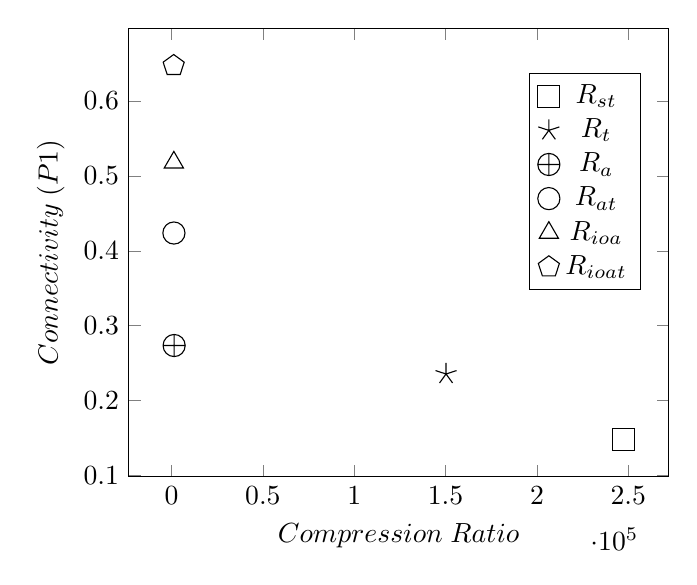
\begin{tikzpicture}
\begin{axis}[
  scatter/classes={
        a={mark=square},%
        b={mark=star},%
        c={mark=oplus},%
        d={mark=o},%
        e={mark=triangle},%
        f={mark=pentagon}
  },
  ylabel=$Connectivity \; (P1)$,
  xlabel=$Compression \; Ratio$,
  mark options={scale=2},
  legend style={at={(.95,0.9)}}
]
\addplot[scatter,only marks,scatter src=explicit symbolic]
coordinates {
% (6.6441, 0.14856667) [a] %0.1301) [a]
% (6.5291, 0.2356) [b] %0.2057) [b]
% (57.4105, 0.2736) [c] %0.2664) [c]
% (65.8846, 0.4238) [d] %0.4221) [d]
% (69.0500, 0.51803333) [e] %0.5169) [e]
% (77.2328, 0.64733333) [f] %0.6598) [f]

(247305.94, 0.14856667) [a]
(150252.41, 0.2356) [b]
(1433.53, 0.2736) [c]
(1314.50, 0.4238) [d]
(1268.24, 0.51803333) [e]
(1184.26, 0.64733333) [f]

};
\legend{$R_{st}$, $R_{t}$, $R_{a}$, $R_{at}$, $R_{ioa}$, $R_{ioat}$}
\end{axis}
\end{tikzpicture}

		}
		\caption{Connectivity precision versus volume ratio.}
		\label{fig:trade-conn-volume}
	\end{subfigure}
	\qquad
	\begin{subfigure}[t]{0.46\textwidth}
		\resizebox{\textwidth}{!}{
			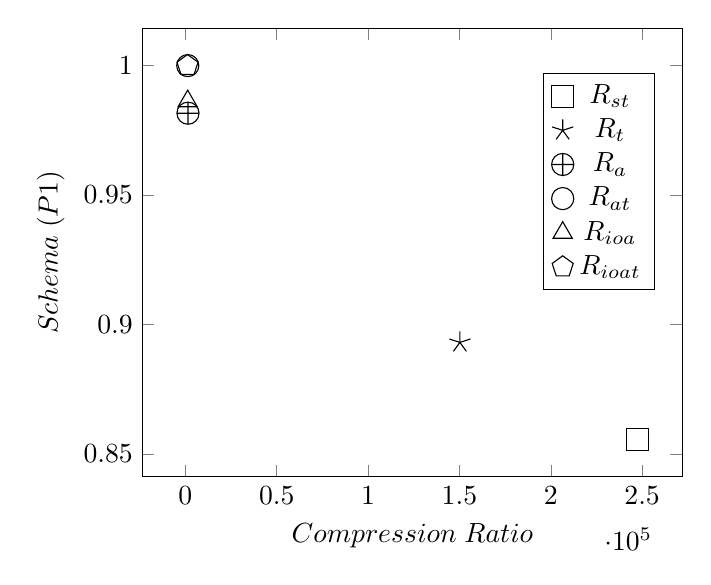
\begin{tikzpicture}
\begin{axis}[
  scatter/classes={
        a={mark=square},%
        b={mark=star},%
        c={mark=oplus},%
        d={mark=o},%
        e={mark=triangle},%
        f={mark=pentagon}
  },
  ylabel=$Schema \; (P1)$,
  xlabel=$Compression \; Ratio$,
  mark options={scale=2},
  legend style={at={(0.95,0.9)}}
]
\addplot[scatter,only marks,scatter src=explicit symbolic]
coordinates {
% (6.6441, 0.85565) [a] %0.6970) [a]
% (6.5291, 0.89303333) [b] %0.8585) [b]
% (57.4105, 0.9816) [c] %0.9733) [c]
% (65.8846, 1.0000) [d]
% (69.0500, 0.98623333) [e] %0.9795) [e]
% (77.2328, 1.0000) [f]

(247305.94, 0.85565) [a]
(150252.41, 0.89303333) [b]
(1433.53, 0.9816) [c]
(1314.50, 1.0000) [d]
(1268.24, 0.98623333) [e]
(1184.26, 1.0000) [f]

};
\legend{$R_{st}$, $R_{t}$, $R_{a}$, $R_{at}$, $R_{ioa}$, $R_{ioat}$}
\end{axis}
\end{tikzpicture}

		}
		\caption{Schema precision versus volume ratio.}
		\label{fig:trade-schema-volume}
	\end{subfigure}
	\qquad%
	\begin{subfigure}[t]{0.46\textwidth}
		\resizebox{\textwidth}{!}{
			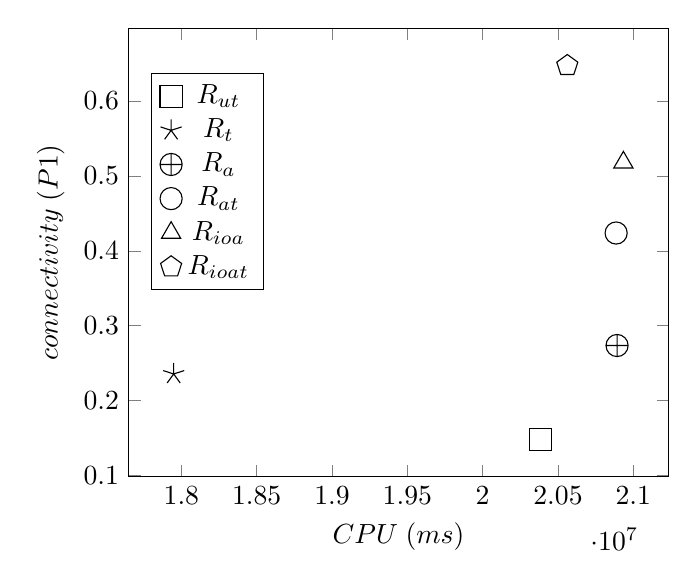
\begin{tikzpicture}
\begin{axis}[
  scatter/classes={
        a={mark=square},%
        b={mark=star},%
        c={mark=oplus},%
        d={mark=o},%
        e={mark=triangle},%
        f={mark=pentagon}
  },
  ylabel=$\gls{connectivity} \; (P1)$,
  xlabel=$CPU \; (ms)$,
  mark options={scale=2},
  legend style={at={(0.25,0.9)}}
]
\addplot[scatter,only marks,scatter src=explicit symbolic]
coordinates {
% (24844125.1190, 0.1301) [a]
% (24669863.0952, 0.2057) [b]
% (24277682.3810, 0.2664) [c]
% (28968841.4286, 0.4221) [d]
% (22053489.7619, 0.5169) [e]
% (22386809.1667, 0.6598) [f]
 (20384066, 0.14856667) [a]
 (17949001, 0.2356) [b]
 (20892062, 0.2736) [c]
 (20885921, 0.4238) [d]
 (20934061, 0.51803333) [e]
 (20561815, 0.64733333) [f]
};
\legend{$R_{ut}$, $R_{t}$, $R_{a}$, $R_{at}$,
 $R_{ioa}$, $R_{ioat}$}
\end{axis}
\end{tikzpicture}

		}
		\caption{Connectivity precision versus summarisation performance.}
		\label{fig:trade-conn-cpu}
	\end{subfigure}
	\qquad%
	\begin{subfigure}[t]{0.46\textwidth}
		\resizebox{\textwidth}{!}{
			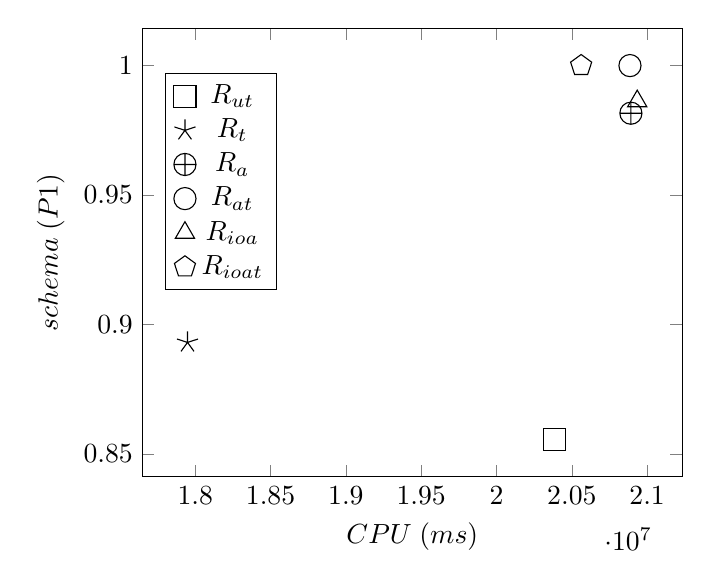
\begin{tikzpicture}
\begin{axis}[
  scatter/classes={
        a={mark=square},%
        b={mark=star},%
        c={mark=oplus},%
        d={mark=o},%
        e={mark=triangle},%
        f={mark=pentagon}
  },
  ylabel=$\gls{schema} \; (P1)$,
  xlabel=$CPU \; (ms)$,
  mark options={scale=2},
  legend style={at={(0.25,0.9)}}
]
\addplot[scatter,only marks,scatter src=explicit symbolic]
coordinates {
% (24844125.1190, 0.6970) [a]
% (24669863.0952, 0.8585) [b]
% (24277682.3810, 0.9733) [c]
%% (28968841.4286, 1.0000) [d]
% (22053489.7619, 0.9795) [e]
% (22386809.1667, 1.0000) [f]

 (20384066, 0.85565) [a]
 (17949001, 0.89303333) [b]
 (20892062, 0.9816) [c]
 (20885921, 1) [d]
 (20934061, 0.98623333) [e]
 (20561815, 1) [f]
};
\legend{$R_{ut}$, $R_{t}$, $R_{a}$, $R_{at}$, $R_{ioa}$, $R_{ioat}$}
\end{axis}
\end{tikzpicture}

		}
		\caption{Schema precision versus summarisation performance.}
		\label{fig:trade-schema-cpu}
	\end{subfigure}
	\caption{Efficiency and precision trade-offs of the candidate summarisation relations. The values are taken as the average across all dataset categories.}
\end{figure}
